\section{Non Equilibrium-Quasi-One-Dimensional flows} 
\label{sec:method}

During the 1950s, The rocket age and the space race age, the rocket nozzles and high enthalpy aerodynamic test facilities, very high and intensive work were done in order to obtain exact numerical solutions for the high temperature gas through the nozzle when the total stagnation temperature increase so much that dissociation occurs or when non-equilibrium take place.

Here are some few examples of how non-equilibrium flow affects the flow physics,

The thrust of the rocket decreases when there is an increase in  temperature of the engine. In hypersonic wind tunnel, the flow of the fluid or air become uncertain

In order to reduce such effects, equilibrium conditions should be met for proper functioning and therefore proper design conditions must be implemented in order for the flow to maintain efficiency.

Until 1969, the nozzle flow solutions were in steady state analysis which were not satisfactory and were not straight forward and now with these chemical equations involved it even becomes more notorious and complicated with involvement of chemical rate equations. The main issue was the saddle point in the throat of the nozzle which made it very difficult to categorize into subsonic and supersonic flow. 

In 1969, a new technique for solving non equilibrium flows are formulated for solving non equilibrium nozzle flows which was formulated by Anderson, The method used a time marching finite difference method. which is was convincingly easy to understand and program in a computer and from there inwards its been prevailing in many nozzle flows and is present up-to date and accepted until the modern days.

Consider Figure 11, The primary assumptions for calculating all the properties on the nozzle grid points, is the assumption of vibrational energy and chemical species concentration as dependant variables.

\begin{figure}[ht]
\centering
  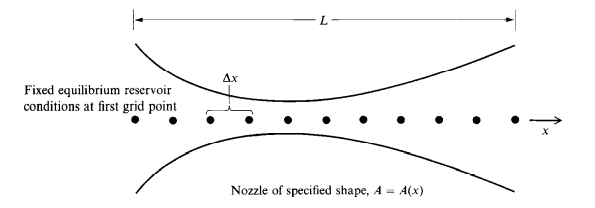
\includegraphics[width=0.7\linewidth]{images/nozzle_timemarching.png}
  \caption{Coordinate system and grid points for time marching of quasi-one-dimensional-flow through a nozzle }
  \label{fig:boat1}
\end{figure}

In Figure 11, The initial conditions that are taken into consideration are as follows for the time marching solution are as follows, The first grid point is considered to be the reservoir conditions, such as total pressure and temperature are considered invariable over time. The values of vibrational energy and c i are guessed and placed arbitrarily in the front node (equilibrium values are recommended). It is required that equilibrium values are assumed till throat section and downstream it is considered frozen flow.

The governing equations for nozzle flows are as follows 

Continuity
\large\[\frac{\partial \rho}{\partial t} = \frac{1}{A} \frac{\partial({\rho U A})}{\partial x}\]
Momentum
\large \[\frac{\partial u}{\partial t} = -\frac{1}{\rho}(\frac{\partial p}{\partial x}+\rho U \frac{\partial u}{\partial x})\]
Energy
\large \[\frac{\partial e}{\partial t} = -\frac{1}{\rho}(P \frac{\partial U}{\partial x}+\rho U \frac{\partial e}{\partial x})+\rho U \frac{\partial \log A}{\partial x})\]
Species continuity equation 
\large \[\frac{\partial e_{vib}}{\partial t} = -\frac{1}{\tau}(e_{vib}^{eq}- e_{vib})- u\frac{\partial e_{vib}}{\partial x})\]
and

\large\[\frac{\partial c_i}{\partial t} = - u \frac{\partial({\rho c_i})}{\partial x}+\frac{w_i}{p}\]
All the above equations are solved step by step in time using the finite difference predictor corrector method, All the flow properties change with time and approach a steady state after a few instances of time. The CFL number that is taken should not exceed the finite rate chemical reactions and non-equilibrium flows that are formed which is clearly defined by the local temperature and pressure in the flow since they dictate the reaction rates. if the chemical reaction rates are very high then below equation dictates the flow

\[\Delta t < \frac{\Delta x}{u+a}\] 